% !TeX document-id = {acd94374-0a5a-4c39-a15c-8f2e56f0151a}
\documentclass[12pt,a4paper, listof=entryprefix, bibliography=totocnumbered,toc=listofnumbered,lof=listofnumbered]{scrartcl}

% WICHTIG!!!
% Pseudokommentar um pdflatex zu erlauben andere Programme zu nutzen z.B. gnuplot
% !TeX TXS-program:compile = txs:///pdflatex/[--shell-escape] 

\usepackage[ngerman]{babel}
\usepackage[utf8]{inputenc}
\usepackage{amsmath}
\usepackage{nccmath}
\usepackage{amsfonts}
\usepackage{amssymb}
\usepackage{graphicx}
\usepackage{fancyhdr}
\usepackage{tabularx}
\usepackage{geometry}
\usepackage{setspace}
\usepackage[right]{eurosym}
\usepackage[printonlyused]{acronym}
\usepackage{subfig}
\usepackage{floatflt}
\usepackage[usenames,dvipsnames]{color}
\usepackage{colortbl}
\usepackage{xcolor}
\usepackage{paralist}
\usepackage{array}
\usepackage{titlesec}
\usepackage{parskip}
\usepackage{picinpar}
\usepackage[pdfpagelabels=true]{hyperref}
\usepackage{listings}
\usepackage{csquotes}
\usepackage{url}
\usepackage{float}
\usepackage{pgfplots}
\usepackage{paralist}
\usepackage[nonumberlist, nogroupskip]{glossaries}

%-----------------------------------------------------------------------------------
% Bibilothek
%-----------------------------------------------------------------------------------
% Einbinden des BibLateX paketes mit Ausgabeeinstellungen
\usepackage[
style=alphabetic,          % Zitierstil
maxbibnames=50,            % alle Autorennamen anzeigen
maxcitenames=4,            % maximale Namen, die im Kürzel angezeigt werden
autocite=inline,           % regelt Aussehen für \autocite (inline=\parancite)
block=space,               % kleiner horizontaler Platz zwischen den Feldern
backref=true,              % Seiten anzeigen, auf denen die Referenz vorkommt
backrefstyle=three+,       % fasst Seiten zusammen, z.B. S. 2f, 6ff, 7-10
date=short,                % Datumsformat
backend = biber,           % Backnend für Aufbereitung
]{biblatex}

%Zusätzliche für Umbrüche für Kleinbuchstaben z.B. in URLs
\appto\UrlBreaks{\do\a\do\b\do\c\do\d\do\e\do\f\do\g\do\h\do\i\do\j
	\do\k\do\l\do\m\do\n\do\o\do\p\do\q\do\r\do\s\do\t\do\u\do\v\do\w
	\do\x\do\y\do\z}


\newcounter{verzeichnis}
\setcounter{verzeichnis}{1}

%Abstände der Einträge
\setlength{\bibitemsep}{1em}     % Abstand zwischen den Literaturangaben
\setlength{\bibhang}{2em}        % Einzug nach jeweils erster Zeile

% Kürzel soll vier Buchstaben der Autoren enthalten statt drei
\DeclareLabelalphaTemplate{
	\labelelement{
		\field[final]{shorthand}
		\field{label}
		\field[strwidth=4,strside=left,ifnames=1]{labelname}
		\field[strwidth=2,strside=left,ifnames=2]{labelname}
		\field[strwidth=1,strside=left]{labelname}
	}
	\labelelement{
		\field[strwidth=2,strside=right]{year}
	}
}

% Bibliothek der Quellen
\bibliography{bib}
\label{bib}

% --------------------------------------------------------------------------------
% Einstellung für Listings
% --------------------------------------------------------------------------------
\lstset{basicstyle=\footnotesize, captionpos=b, breaklines=true, showstringspaces=false, tabsize=2, frame=lines, numbers=left, numberstyle=\tiny, xleftmargin=2em, framexleftmargin=2em}
\makeatletter
\def\l@lstlisting#1#2{\@dottedtocline{1}{0em}{1em}{\hspace{1,5em} Lst. #1}{#2}}
\makeatother

% --------------------------------------------------------------------------------
% Seitenformate
% --------------------------------------------------------------------------------
%Seitenformat
\geometry{a4paper, top=27mm, left=30mm, right=20mm, bottom=32mm, headsep=12mm, footskip=12mm}

% --------------------------------------------------------------------------------
% Metainformationen
% --------------------------------------------------------------------------------
\hypersetup{unicode=false, pdftoolbar=true, pdfmenubar=true, pdffitwindow=false, pdfstartview={FitH},
	pdftitle={Vorlage},
	pdfauthor={Stefan Jung},
	pdfsubject={Abschlussarbeit},
	pdfcreator={\LaTeX\ with package \flqq hyperref\frqq},
	pdfproducer={pdfTeX \the\pdftexversion.\pdftexrevision},
	pdfkeywords={Vorlage},
	pdfnewwindow=true,
	colorlinks=true,linkcolor=black,citecolor=black,filecolor=magenta,urlcolor=black}
\pdfinfo{/CreationDate (D:20141024101000)}
%\pgfplotsset{compat=1.11}

%-----------------------------------------------------------------------------------
% Abkürzungen AKRONYME HIER ERGÄNZEN
%-----------------------------------------------------------------------------------
\glssetwidest{SMPLSP}% Längste Abkürzung für eine korrekte Einrückung

\makenoidxglossaries %Leeres Verzeichnis erstellen

%Abkürzungen hinzufügen
\newacronym{LIP}{LIP}{Labor für Informationstechnik und Produktionslogistik}
\newacronym{OTH}{OTHR}{Ostbayerische Technische Hochschule Regensburg}
\newacronym{CSS}{CSS}{Cascading Style Sheets}
\newacronym{SMPLSP}{SMPLSP}{Static Multi-product  Proportional Lotsizing and Scheduling Problem}
\newacronym{XML}{XML}{Extensible Markup Language}
\newacronym{CSV}{CSV}{Comma-separated values}
\newacronym{GUI}{GUI}{Graphical User Interface}

\begin{document}
% --------------------------------------------------------------------------------
% Globale Formateinstellungen
% --------------------------------------------------------------------------------
\onehalfspacing
% Abstände Überschrift
\titlespacing{\section}{0pt}{42pt}{6pt}
\titlespacing{\subsection}{0pt}{12pt}{6pt}
\titlespacing{\subsubsection}{0pt}{12pt}{6pt}

% Kopf- und Fusszeile
\pagestyle{fancy}
\lhead{}\chead{}
\rhead{\thesection\space\contentsname}
\lhead{}\cfoot{}
\rfoot{\ \linebreak \thepage}
\renewcommand{\headrulewidth}{0.4pt}
\renewcommand{\footrulewidth}{0.4pt}

% Nummereriung
\renewcommand{\thesection}{\Roman{section}}
\renewcommand{\theHsection}{\Roman{section}}
\pagenumbering{Roman}

% eigene Farbdefinitionen
\definecolor{lip}{HTML}{3366FF}
\definecolor{grey}{HTML}{ABABAB}

% ---------------------------------------------------------------------------
% Titelseite
% ---------------------------------------------------------------------------
\thispagestyle{empty}

%LIP Schriftzug in eigener Farbe 
\textsf{\begin{minipage}{.69\textwidth}
	\large
	\textcolor{lip}{\textbf{Labor für Informationstechnik und\\Produktionslogistik (LIP)}} %Farbe setzten
	\small 
	\textbf{\\Verfahren, Strategien, Prozesse und IT-Systeme}
	\\Professor Dr.-Ing. Frank Herrmann
\end{minipage}
%Einbinden des OTH Logos mir rechtsbündiger Ausrichtung
\begin{minipage}{.29\textwidth}
	\begin{flushright}
		
\includegraphics[scale=.15]{Bilder/othlogo}\\
	\end{flushright}
\end{minipage}}
 
% Zeilenabstand
\onehalfspacing	

%Beschriftung der Titelseite
\begin{center}

	\vspace*{4cm} %4 cm Vorspann
	\Large
	\textbf{Entwicklerhandbuch zur Losgrößen- und Ressourceneinsatzplanung bei Fließproduktion}\\ %Titel der Arbeit
	\large
	\textbf{Klassisches Losgrößenmodell, Mehrproduktproduktion}\\ %Untertitel der Arbeit
		
	\vspace*{8cm} %8 cm Vorspann
	\normalsize
	\begin{center}
	Juni 2015\\
	\textbf{Arnold Christiane \\ Denzin Timo \\ Eichinger Tobias \\ Sonnleitner Daniel \\ Wagner Pilar} %Name des Autors
	
	\end{center}
\end{center}
\pagebreak

% ------------------------------------------------------------------------------
% Inhaltsverzeichnis
% ------------------------------------------------------------------------------
% Inhaltsverzeichnis
\singlespacing %Zeilenabsatnd reduzieren
\setcounter{section}{0}
\setcounter{page}{1}
\addcontentsline{toc}{section}{Inhaltsverzeichnis}%hinzufügen des Inhaltsverzeichnises selbst

\tableofcontents %Ausgabe des Inhaltsverzeichnisses
\pagebreak

% ------------------------------------------------------------------------------
% Setzen der Nummerierungen für Normaltext
% ------------------------------------------------------------------------------
\onehalfspacing %Zeilenabstand auf 1.5
\renewcommand{\thesection}{\arabic{section}} %Arabische Beschriftung für Absatznummern
\pagenumbering{arabic}  %Seitennummerrierung auf arabisch setzten
\setcounter{page}{1}	%Seitenzahl für Inhalt auf 1 setzten
\setcounter{section}{0}
% Kopfzeile mit aktuellem Hauptkapitel darstellen
\renewcommand{\sectionmark}[1]{\markright{#1}} %Section ausgeben
\renewcommand{\subsectionmark}[1]{}            %Subsection nicht ausgeben
\renewcommand{\subsubsectionmark}[1]{}         %Subsubsection nicht ausgeben
\rhead{\rightmark}                             %Ausgabe Rechtsbündig

%------------------------------------------------------------------------------
%	Einführung
%------------------------------------------------------------------------------
\section{Einführung}
Das vorliegende Dokument ist ein Handbuch für Entwickler des \textit{"\gls{SMPLSP}"}-Tools zur Losgrößen- und Ressourceneinsatzplanung bei Fließproduktion. 
\\
Die Software ist in Java 8 geschrieben und die Benutzeroberfläche wurde mittels JavaFX 8 realisiert.
\\
Das folgende Bild zeigt die Software.

\begin{figure}[H]
	\centering
	\includegraphics[width=1.0\linewidth]{Bilder/smplsp.png} 
	\captionof{figure}[]{Oberfläche des SMPLSP-Tools}
	\label{fig:osgi}
\end{figure}

\subsection{Aufbau des Dokuments}
Zu Beginn soll die Problemstellung erklärt und der Ablauf des hier verwendeten Verfahrens erläutert werden.
\\
Anschließend folgt eine kurze Beschreibung der Funktionen der Software.
\\
Unter dem Punkt Aufbau der Software sollen die einzelnen Komponenten erläutert werden.
\\
Im letzten Kapitel wird auf die Implementierung der einzelnen Komponenten eingegangen.
\subsection{Problemstellung}
Das vorliegende Programm dient zur Losgrößen- und Ressourceneinsatzplanung bei Fließproduktion. Dabei werden sowohl die Produktionszyklen für ein einzelnes Produkt, als auch der gemeinsame Zyklus für mehrere Produkte berechnet.
\subsection{Beschreibung der Software}
Nach dem Start des Tools müssen die Daten zur Berechnung eingegeben werden. Dies geschieht entweder manuell oder durch das Laden einer Datei. Es wird der Import von \gls{CSV}-Dateien unterstützt.
\\
Nachdem die Produktionszyklen berechnet wurden, werden in den verschiedenen Reitern der Oberfläche die Ergebnisse in Form von Tabellen und Diagrammen dargestellt. Bei einem Klick in eine Tabellenzeile, erscheinen in der Erklärkomponente Details zur Berechnung dieses Wertes.
\\
Detailliertere Information über die Funktionen der Software finden Sie im Benutzerhandbuch.


%------------------------------------------------------------------------------
%	Aufbau der Software
%------------------------------------------------------------------------------

\section{Aufbau der Software}
Im Folgenden werden die verwendete Technik und die Komponenten des Programms vorgestellt. Die Komponenten werden durch Packages realisiert, daher werden in dieser Dokumentation auch die Packagenamen verwendet. Im weiteren Verlauf werden die Begriffe Komponente und Package gleichbedeutend benutzt.

\subsection{Verwendete Techniken}
\paragraph{JavaFX 8}
Die Benutzeroberfläche der Software wurde in JavaFX 8 entwickelt. JavaFX verwendet das Model-View-Controller Prinzip.
\\
Um die Gestaltung des \gls{GUI} zu vereinfachen, wird der SceneBuilder verwendet. Der SceneBuilder ist ein Tool zur einfachen Erstellung von JavaFX Layouts. Dabei muss kein Code geschrieben werden, da dies vom SceneBuilder übernommen wird. Das folgende Bild zeigt den SceneBuilder.

\begin{figure}[H]
	\centering
	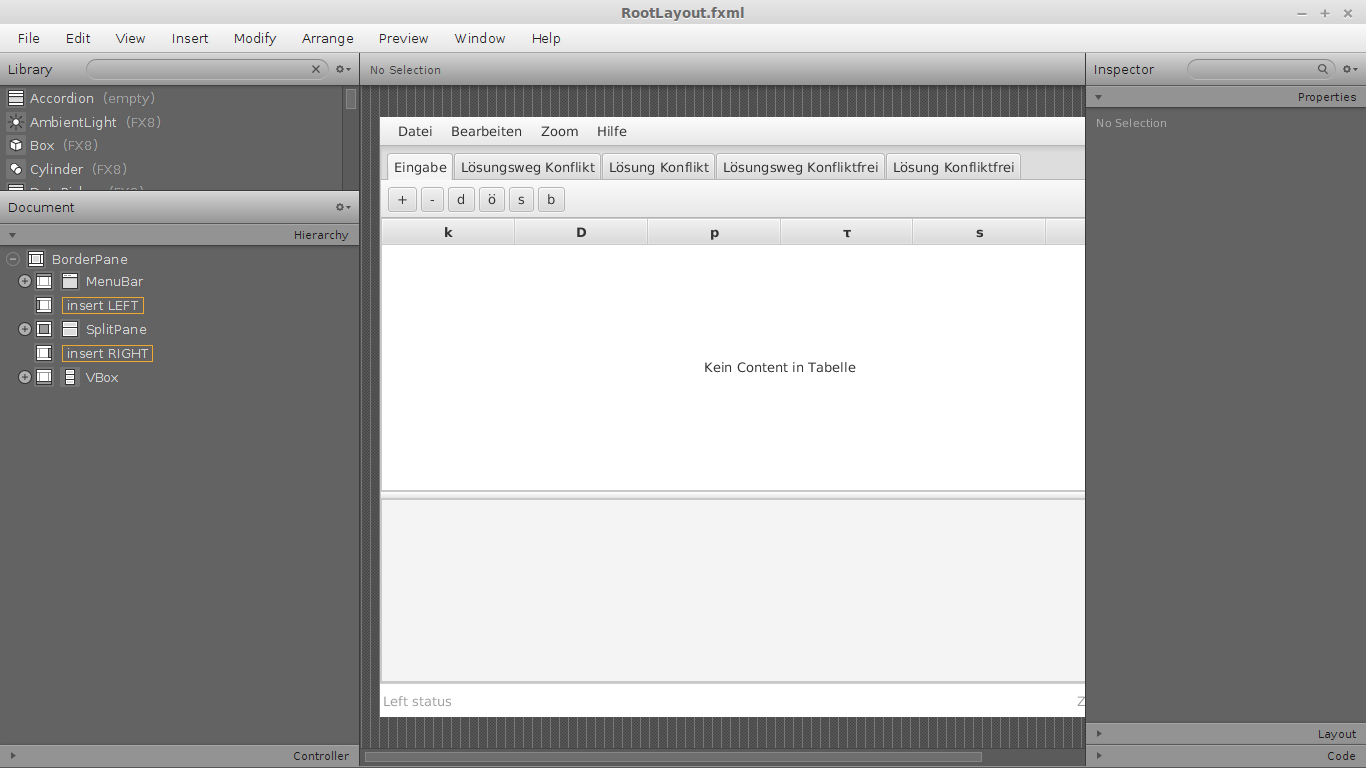
\includegraphics[width=1.0\linewidth]{Bilder/scenebuilder.png} 
	\captionof{figure}[]{Der SceneBuilder}
	\label{fig:osgi}
\end{figure}

Beim Model-View-Controller Prinzip enthält die View lediglich den grafischen Aufbau der Oberfläche. Dieser Aufbau wird einer speziellen \gls{XML} Datei gespeichert, einer sogenannten FXML Datei. 
\\
Eine zugehörige Controller Klasse implementiert die, zur View gehörige, Logik in einer Java Klasse. 
\\
Im Model werden die verwendeten Daten abgespeichert und verwaltet. 
\\
Weder Model noch View enthalten Logik. Dies führt zu einer sauberen Schichtentrennung zwischen Benutzeroberfläche (View), Logik (Controller) und Datenhaltung (Model).
\\
\\
In der FXML-Datei wird die Controller Klasse gesetzt, dadurch kann der Compiler, beim Übersetzten des Programms, Controller und View einander zuordnen. 
Im Folgenden ist zu sehen, wie dies im SceneBuilder umgesetzt werden kann.

\begin{figure}[H]
	\centering
	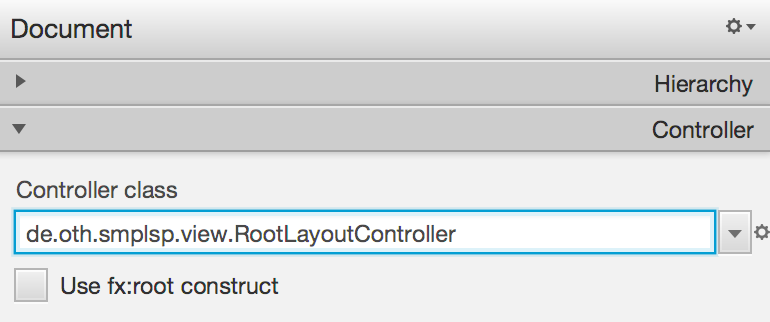
\includegraphics[]{Bilder/controller_setzen.png} 
	\captionof{figure}[]{Controller Klasse im SceneBuilder setzten}
	\label{fig:osgi}
\end{figure}

Um auf die Elemente der \gls{GUI} vom Controller aus zuzugreifen, werden beim Deklarieren eines Elements die @FXML Annotation gesetzt. Zusätzlich wird in der FXML-Datei die fx:id des Elements vergeben. Diese muss mit der Bezeichnung im Controller übereinstimmen. 
\\
In der folgenden Abbildung ist zu sehen, wie im SceneBuilder die fx:id gesetzt wird.

\begin{figure}[H]
	\centering
	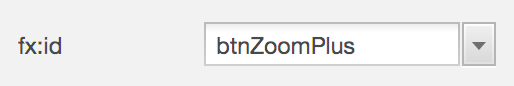
\includegraphics[]{Bilder/fxid.png} 
	\captionof{figure}[]{Setzten der fx:id im SceneBuilder}
	\label{fig:osgi}
\end{figure}

Und hier das Beispiel im Code:
\begin{lstlisting}[caption= Beispielprogramm, label=lst:code]
	// Code ...
	
	@FXML
	private Button btnZoomPlus; 
	
	// Code...
\end{lstlisting}

Weitere Informationen finden Sie in diesem Tutorial zu JavaFX.
\\
(http://code.makery.ch/library/javafx-8-tutorial/)

\paragraph{JFreeChart}
Zur Visualisierung der Losgrößen wird das Java-Framework JFreeChart verwendet. Mit JFreeChart können verschiedene Diagramme erstellt werden, darunter auch die hier verwendeten Gantt-Diagramme. 

\paragraph{JUnit}
Um die implementierte Logik automatisiert testen zu können, werden JUnit - Tests verwendet. Dabei wird eine eigene Testklasse geschrieben, die feste Eingabedaten enthält. Anschließend wird die zu testende Methode ausgeführt und die Rückgabewerte der Methode automatisiert mit den erwarteten Ausgabedaten verglichen. Stimmen sie überein, war der Test erfolgreich.
\\
Dies ermöglicht vor allem bei größeren Methoden ein Testen ohne Zutun des Entwicklers.

\subsection{Komponenten}
\paragraph{algorithms}
Hier sind die Algorithmen zur Berechnung der Losgrößen implementiert. Es gibt jeweils eine Klasse zur Berechnung der klassischen Losgrößen und zur Berechnung der Mehrproduktlosgrößen. Beide Klassen implementierten ein Interface, das gemeinsame Methoden vorgibt. 
\\
Der Produktionsprozess wird in beiden Fällen gleich berechnet, deshalb wird hierfür die selbe Klasse verwendet.
\paragraph{formula}
Die Komponente formula enthält die Klassen zur Erzeugung der Formeln, die in der Erklärkomponente angezeigt werden sollen. Die hierbei erzeugten Strings enthalten die mathematischen Formeln, in Form von \LaTeX - Code. Diese werden dynamisch zur Laufzeit erzeugt und mit den passenden Daten gefüllt. Damit ist es möglich, zu jedem Ergebnis eine Formel mit eingesetzten Werten zu erzeugen.
\\
Für die Formeln der klassischen Losgrößen und der Mehrproduktlosgrößen ist jeweils eine eigene Klasse implementiert. Außerdem ist noch eine Klasse für die Formeln des Produktionsprozesses und für produktspezifische Formeln vorhanden.
\paragraph{messages}
Dieses Package verwaltet die angezeigten Texte und Beschriftungen der Software. Dabei wird ein Ressource Handler verwendet, der es zusätzlich ermöglicht, das Programm in eine andere Sprache zu übersetzen, ohne große Änderungen am Code vorzunehmen.
\paragraph{persistence}
Hier werden die Dateizugriffe verwaltet. Hierfür wird für jeden Dateityp eine eigene Klasse erstellt, die von der Klasse AbstractFile erbt. Dadurch müssen Funktionen wie das Laden der Datei nicht erneut implementiert werden.
\paragraph{util}
In dieser Komponente werden, neben einigen Hilfsklassen, vor allem die Einstellungen des Tools verwaltet. Hierfür wurde eine Singleton Klasse Configuration geschaffen.
\paragraph{zoom}
In der Komponente zoom sind die Klassen zum Vergrößern und Verkleinern der Benutzeroberfläche enthalten. Dies wird mittels Veränderungen in den \gls{CSS} realisiert.
\paragraph{error}
Hier werden die Exceptions und andere Fehlermeldungen verwaltet.
\paragraph{model}
Die Model - Klassen zur Datenhaltung werden in diesem Package aufbewahrt. Dazu gehören die Abstraktionen von Produkt, Produktionsprozess und dem Ergebnis der Analyse.
\paragraph{test}
Die Komponente test enthält die Klassen zur Durchführung der JUnit - Tests. 
\paragraph{view}
In dieser Komponente befinden sich die Controller und FXML Dateien der grafischen Oberfläche. Diese ist in ein RootLayout und die fünf Reiter unterteilt. Das RootLayout definiert hier den Rahmen für die Reiter, die Menüleiste und die Unterleiste der Applikation.
\\
Die Reiter sind in das RootLayout integriert, besitzen aber eigene FXML-Dateien und Controller-Klassen. Dies wird im SceneBuilder wie folgt dargestellt:

\begin{figure}[H]
	\centering
	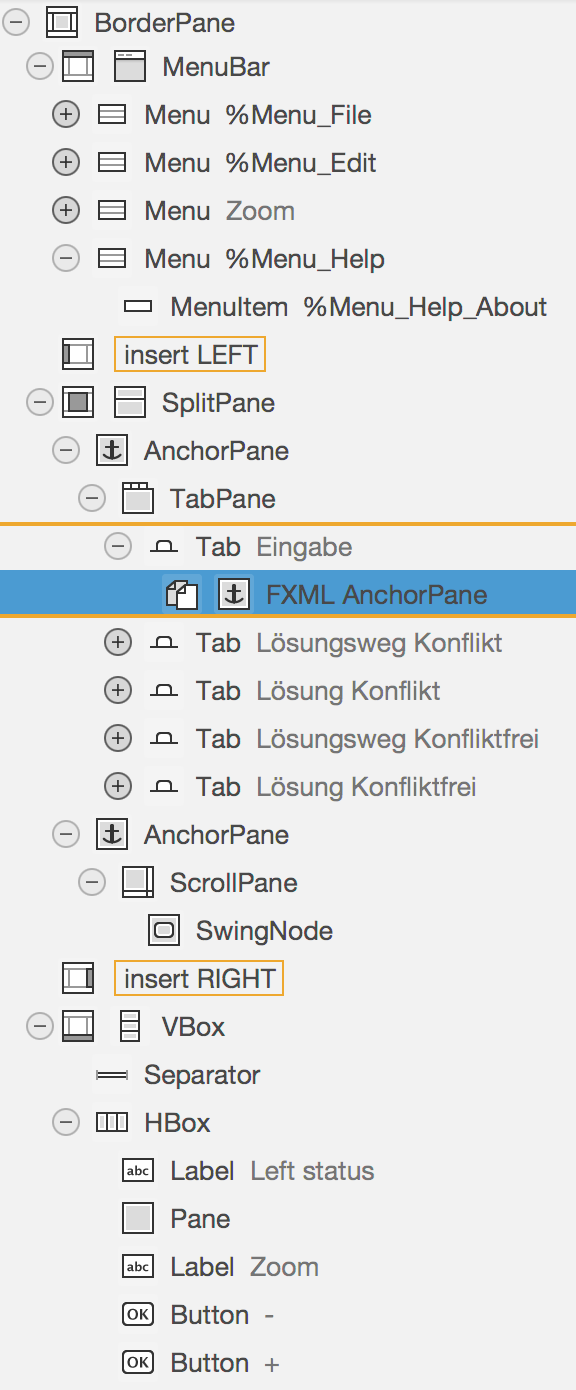
\includegraphics[]{Bilder/tabs.png} 
	\captionof{figure}[]{Darstellung der Reiter im SceneBuilder}
	\label{fig:osgi}
\end{figure}

Damit die Unterkomponenten des RootLayout miteinander kommunizieren und aufeinander zugreifen können, wird ihnen der RootLayoutController übergeben. Dadurch ist es ihnen möglich auf die Elemente und Teile des RootLayout zuzugreifen.
\\\\
Nachfolgend sind die einzelnen Komponenten im Package - Explorer zu sehen.

\begin{figure}[H]
	\centering
	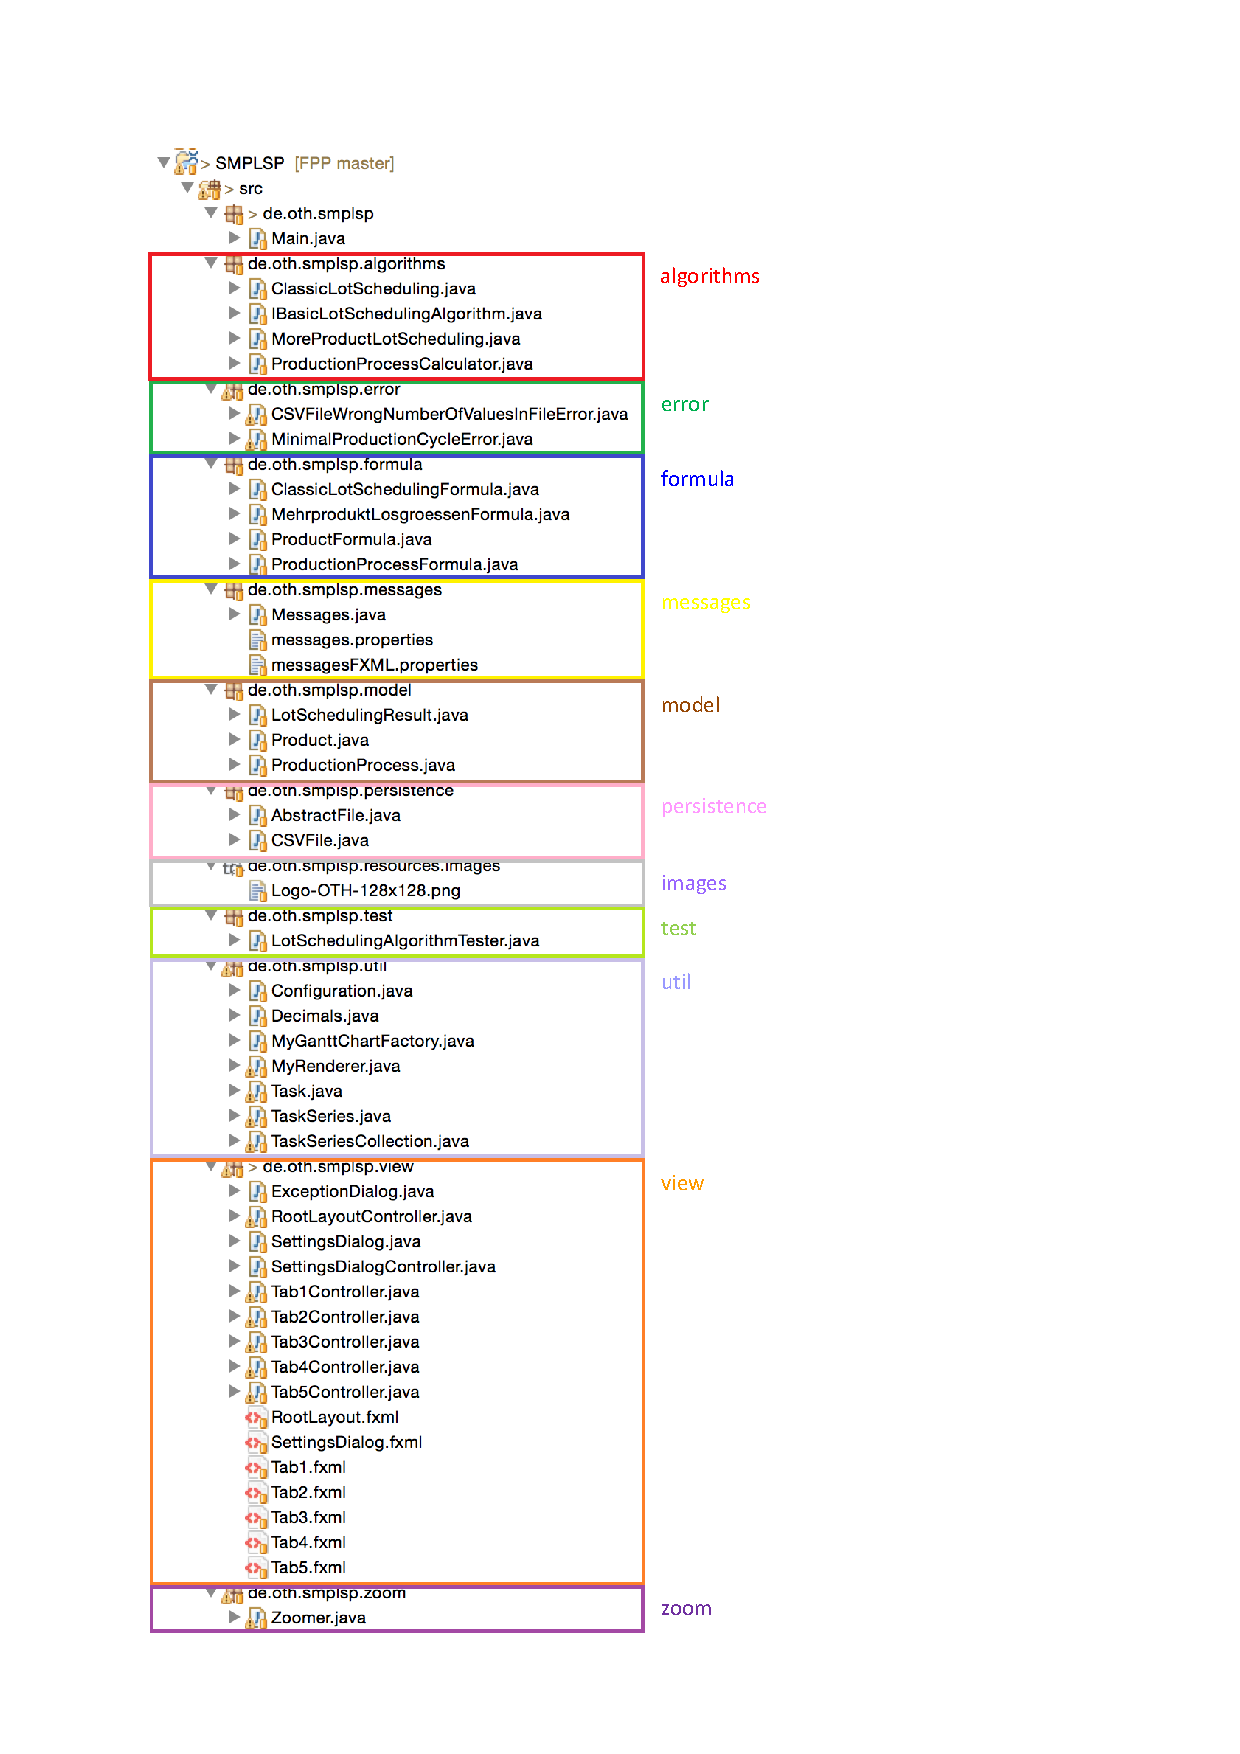
\includegraphics[width=0.8\linewidth]{Bilder/packages_beschriftet.pdf} 
	\captionof{figure}[]{Komponenten im Package - Explorer}
	\label{fig:osgi}
\end{figure}

%------------------------------------------------------------------------------
%	Implementierung
%------------------------------------------------------------------------------

\section{Implementierung}
Dieses Kapitel beschreibt die Implementierung, sowie die bei der Entwicklung der Komponenten verwendeten Bibliotheken. Dabei wird vor allem auf die Algorithmen der Losgrößenberechnung eingegangen. Die einzelnen Klassen werden in der Javadoc beschrieben.
 
\subsection{Verwendete Bibliotheken}
Die verwendeten Bibliotheken sind im Ordner lib gespeichert, um einen pfadunabhängigen Import in den Java Build Path zu ermöglichen. 
\\
Sie unterteilen sich in fünf Einsatzbereiche:
\begin{itemize}
	\item[CSV-Import:] Diese Bibliotheken bieten Klassen zum automatisierten Einlesen und Beschreiben von \gls{CSV}-Dateien an. Dies wird mittels einer Parser und einer Printer Klasse erreicht.
	\item[JavaFX Zusätze:] Die hier verwendeten Bibliotheken erweitern JavaFX um vorgefertigte Dialoge und Buttons.
	\item[JFreeChart:] Das Einbinden dieser Bibliotheken ermöglicht es Daten mittels Diagrammen zu visualisieren. Dabei wird die Klasse JFreeChart mit Daten gefüllt und dann zur Anzeige gebracht.
	\item[\LaTeX :] Die Formeln in der Erklärkomponente werden mittels \LaTeX - Code erzeugt. Der zur Verfügung gestellten Klasse TeXFormula wird der \LaTeX - Code übergeben und daraus ein Bild generiert.
	\item[Resource Handler:] Der Resource Handler ersetzt die Eclipse eigene Funktion Source $\rightarrow$ Externalize Strings. Diese dient zur Auslagerung der Strings im Java Code in eine eigene Properties Datei. Dies hat den Vorteil, dass der Code übersichtlicher wird und die Texte in mehrere Sprachen übersetzt werden können, ohne in den Klassen etwas zu ändern.
\end{itemize}

Nachfolgende Abbildung zeigt die verwendeten Bibliotheken in der Ordnerstruktur.
\begin{figure}[H]
	\centering
	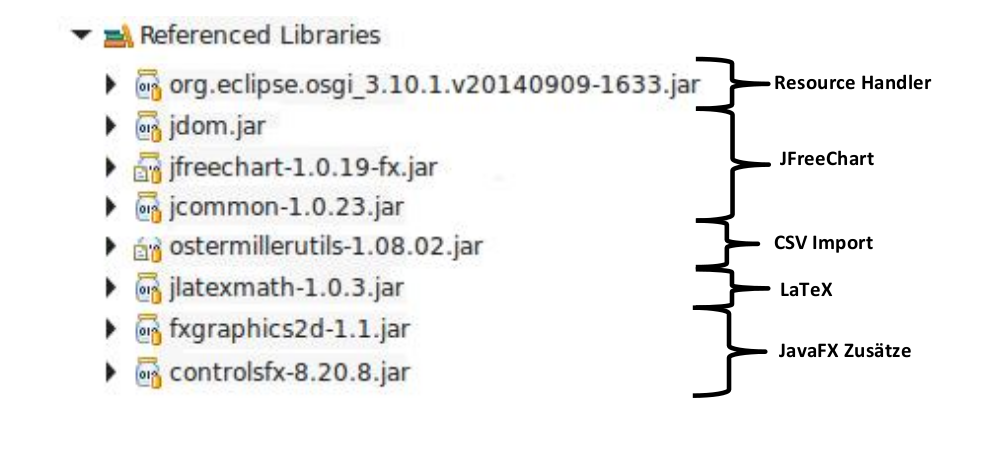
\includegraphics[width=0.9\linewidth]{Bilder/libraries_beschriftet.png} 
	\captionof{figure}[]{Verwendete Bibliotheken}
	\label{fig:osgi}
\end{figure}

\subsection{JFreeChart}
Die Diagramme in Reiter 3 und Reiter 5 wurden mit JFreeChart realisiert. 
\\
Da die übergebenen Start- und Endwerte der einzelnen Balken Gleitkommazahlen sind, JfreeChart aber standardmäßig nur mit Date- oder Integerwerten umgehen kann, mussten einige JfreeChart Klassen angepasst werden. Diese veränderten Klassen sind im package util zu finden. Nachfolgende Abbildung zeigt dieses im Packageexplorer.

\begin{figure}[H]
	\centering
	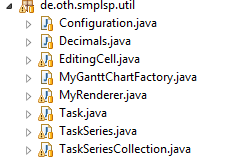
\includegraphics[width=0.5\linewidth]{Bilder/util_package.png} 
	\captionof{figure}[]{Veränderte Klassen für JFreechart}
	\label{fig:osgi}
\end{figure}

Die Klassen Task, TaskSeries und TaskSeriesCollection wurden verändert, um mit Gleitkommazahlen umgehen zu können. 
\\
Die Klasse MyRenderer übernimmt die richtige Farbgebung der Balken innerhalb der Charts.
In MyGanttChartFactory werden die Achsen beschriftet, die Legende des Charts erzeugt und die Hintergrundfarbe festgelegt.
\\
Sämtliche benötigten Methoden und Klassen werden aus dem Controller der jeweiligen View aufgerufen. Der Methode createDataset wird die Liste der Produktionsprozesse aus dem Controller übergeben und daraus eine TaskSeriesCollection erzeugt. Wichtig hierbei ist, dass jede Zeile einen Task darstellt und die Balken für Rüst- und Produktionszeit in einem Subtask abgebildet werden. Alle Subtasks werden dann dem übergeordneten Task hinzugefügt. Abschließend werden alle Tasks zu einer TaskSeries hinzugefügt und diese in eine TaskSeriesCollection aufgenommen. Diese endgültige TaskSeriesCollection wird nun mittels showChart und createChart an die oben beschriebene MyGanttChartFactory übergeben. Diese erstellt daraus ein Gantt Chart und zeigt dieses in der Benutzeroberfläche an.
\subsection{Zoomen}
Die Zoomfunktion wird wird über die Klasse Zoomer im Package zoom gesteuert. Dort sind verschiedene Schriftgrößen definiert (Schriftgröße für Standard-Fonts, Schriftgröße für die Latex-Fonts (Erklärkomponente) und Schriftgröße für das JFreeChart).
\\
Die verschiedenen Komponenten der Oberfläche werden wie folgt skaliert:
\begin{itemize}
	\item Für die verwendeten Icon-Fonts werden die Icons in der neuen Schiftgröße neu berechnet.
	\item Bei den JFreeChart Diagrammen wird analog verfahren.
	\item Der Inhalt der Erklärkomponente wird ebenfalls mit der neuen Schriftgröße neu berechnet.
	\item Für die restlichen \gls{GUI}-Elemente erfolgt eine Modifikation des verwendeten CSS-Styles. Hierbei wird die \gls{CSS}-Style-fx-font-size mit der neuen Schriftgröße gesetzt und geladen.
\end{itemize}

\subsection{Algorithmen}
In diesem Programm werden zwei verschiedene Verfahren verwendet. Die klassische Losgrößenberechnung und die Mehrproduktlosgrößenberechnung. Zur Verdeutlichung wird Pseudocode verwendet.
\subsubsection{Klassiche Losgrößenberechnung}
Zu Beginn findet die Losgrößenberechnung für ein Produkt statt. Diese ist in fünf Schritte unterteilt:
\begin{enumerate}
	\item Berechne die Lose für jedes Produkt
	\item Berechne die Produktionszeit für jedes Produkt
	\item Berechne die Effizienz der Maschine
	\item Berechne den optimalen Produktionszyklus für jedes Produkt
	\item Berechne die Reichweite für die einzelnen Produkte
\end{enumerate}
Nachfolgend ist der Ablauf in Pseudocode dargestellt.
\begin{lstlisting}[caption= Beispielprogramm, label=lst:code]
classicLotScheduling(List<Product> products){

    Map<Integer, Double> tOptSingle = new HashMap<Integer, Double>();
    LotSchedulingResult result;

	// calculateBatchSize 1
	for (Product product : products) {
	    product.setQ(Math.sqrt((2 * product.getD() * product.getS())
		    / (product.getH() * (1 - (product.getD() / product.getP())))));
	}
	// calculateProductionTime 2
	for (Product product : products) {
	    product.setT(product.getQ() / product.getP());
	}
	// calculateEfficiencyOfMachine 3
	for (Product product : products) {
	    product.setRoh(product.getD() / product.getP());
	}
	// calculateOptProductionCycle 4
	for (Product product : products) {
	    tOptSingle.put(
		    product.getK(),
		    Math.sqrt((2 * product.getS() / (product.getH()
	}
	// calculateRange 5
	for (Product product : products) {
	    product.setR(product.getQ() / product.getD());
	}
	return new LotSchedulingResult(products, tOptSingle);
}
\end{lstlisting}

\subsubsection{Mehrproduktlosgrößen}
Im zweiten Durchlauf findet die Losgrößenberechnung für mehrere Produkt statt. Diese ist in sechs Schritte unterteilt:
\begin{enumerate}
	\item Berechne die Effizienz der Maschine
	\item Berechne den Produktionszyklus für die Produkte
	\item Berechne den minimalen Produktionszyklus
	\item Berechne den optimalen gemeinsamen Produktionszyklus
	\item Berechne die Produktionszeit für jedes Produkt
	\item Berechne die Reichweite für die einzelnen Produkte
\end{enumerate}
Nachfolgend ist der Ablauf in Pseudocode dargestellt.
\begin{lstlisting}[caption= Beispielprogramm, label=lst:code]
MoreProductLotScheduling(List<Product> products){
	
    LotSchedulingResult result;
    Double tOpt;
	Double tMin;

	// calculateEfficiencyOfMachine 1
	for (Product product : products) {
	    product.setRoh(product.getD() / product.getP());
	}

	// calculateOptProductionCycle 2
	double numerator = 0.0;
	double denominator = 0.0;

	for (Product product : products) {
	    numerator += product.getS();
	}

	numerator *= 2;

	for (Product product : products) {
	    denominator += (product.getH() * product.getD() * (1 - product
		    .getRoh()));
	}

	tOpt = Math.sqrt(numerator / denominator);

	// calculateMinProductionCycle 3
	double numerator = 0.0;
	double denominator = 0.0;

	for (Product product : products) {
	    numerator += product.getTau();
	}

	for (Product product : products) {
	    denominator += product.getRoh();
	}

	denominator = 1 - denominator;

	tMin = (numerator / denominator);

	if (tOpt < tMin) {
	    throw new MinimalProductionCycleError();
	}

	// calculateBatchSize 4
	for (Product product : products) {
	    product.setQ(product.getD() * tOpt);
	}

	// calculateProductionTime 5
	for (Product product : products) {
	    product.setT(product.getQ() / product.getP());
	}

	// calculateRange 6
	for (Product product : products) {
	    product.setR(product.getQ() / product.getD());
	}

	return new LotSchedulingResult(products, tOpt, tMin);
}
\end{lstlisting}
%-------------------------------------------------------------------------------------
% Verzeichnisse %-------------------------------------------------------------------------------------
%	\rhead{Verzeichnisse} %Kopftextbeschriftung
%
%	\stepcounter{section}
%	\phantomsection \label{Verzeichnisse}
%	\addcontentsline{toc}{section}{Verzeichnisse} %Ohne Nummer ins Inhaltsverzeichnis
%	\renewcommand{\thesection}{\Roman{verzeichnis}}
	
	% Abkürzungen
%	\stepcounter{verzeichnis}
	\newpage
	\section{Abkürzungsverzeichnis}
	\vspace{-6em} % Abstand analog der anderen Verzeichnisse reduzieren
	\printnoidxglossary[type=\acronymtype,style=alttree,title=,toctitle=] %automatischen Titel und Gliederungsbeschriftung unterdrücken - sonst steht da Glossarie
	


\end{document}
